\documentclass[journal,12pt,twocolumn]{IEEEtran}

\usepackage{setspace}
\usepackage{gensymb}
\singlespacing
\usepackage[cmex10]{amsmath}

\usepackage{amsthm}

\usepackage{mathrsfs}
\usepackage{txfonts}
\usepackage{stfloats}
\usepackage{bm}
\usepackage{cite}
\usepackage{cases}
\usepackage{subfig}

\usepackage{longtable}
\usepackage{multirow}

\usepackage{enumitem}
\usepackage{mathtools}
\usepackage{steinmetz}
\usepackage{tikz}
\usepackage{circuitikz}
\usepackage{verbatim}
\usepackage{tfrupee}
\usepackage[breaklinks=true]{hyperref}
\usepackage{graphicx}
\usepackage{tkz-euclide}

\usetikzlibrary{calc,math}
\usepackage{listings}
    \usepackage{color}                                            %%
    \usepackage{array}                                            %%
    \usepackage{longtable}                                        %%
    \usepackage{calc}                                             %%
    \usepackage{multirow}                                         %%
    \usepackage{hhline}                                           %%
    \usepackage{ifthen}                                           %%
    \usepackage{lscape}     
\usepackage{multicol}
\usepackage{chngcntr}

\DeclareMathOperator*{\Res}{Res}

\renewcommand\thesection{\arabic{section}}
\renewcommand\thesubsection{\thesection.\arabic{subsection}}
\renewcommand\thesubsubsection{\thesubsection.\arabic{subsubsection}}

\renewcommand\thesectiondis{\arabic{section}}
\renewcommand\thesubsectiondis{\thesectiondis.\arabic{subsection}}
\renewcommand\thesubsubsectiondis{\thesubsectiondis.\arabic{subsubsection}}


\hyphenation{op-tical net-works semi-conduc-tor}
\def\inputGnumericTable{}                                 %%

\lstset{
%language=C,
frame=single, 
breaklines=true,
columns=fullflexible
}
\begin{document}


\newtheorem{theorem}{Theorem}[section]
\newtheorem{problem}{Problem}
\newtheorem{proposition}{Proposition}[section]
\newtheorem{lemma}{Lemma}[section]
\newtheorem{corollary}[theorem]{Corollary}
\newtheorem{example}{Example}[section]
\newtheorem{definition}[problem]{Definition}

\newcommand{\BEQA}{\begin{eqnarray}}
\newcommand{\EEQA}{\end{eqnarray}}
\newcommand{\define}{\stackrel{\triangle}{=}}
\bibliographystyle{IEEEtran}
\raggedbottom
\setlength{\parindent}{0pt}
\providecommand{\mbf}{\mathbf}
\providecommand{\pr}[1]{\ensuremath{\Pr\left(#1\right)}}
\providecommand{\qfunc}[1]{\ensuremath{Q\left(#1\right)}}
\providecommand{\sbrak}[1]{\ensuremath{{}\left[#1\right]}}
\providecommand{\lsbrak}[1]{\ensuremath{{}\left[#1\right.}}
\providecommand{\rsbrak}[1]{\ensuremath{{}\left.#1\right]}}
\providecommand{\brak}[1]{\ensuremath{\left(#1\right)}}
\providecommand{\lbrak}[1]{\ensuremath{\left(#1\right.}}
\providecommand{\rbrak}[1]{\ensuremath{\left.#1\right)}}
\providecommand{\cbrak}[1]{\ensuremath{\left\{#1\right\}}}
\providecommand{\lcbrak}[1]{\ensuremath{\left\{#1\right.}}
\providecommand{\rcbrak}[1]{\ensuremath{\left.#1\right\}}}
\theoremstyle{remark}
\newtheorem{rem}{Remark}
\newcommand{\sgn}{\mathop{\mathrm{sgn}}}
%\providecommand{\abs}[1]{\left\vert#1\right\vert}
\providecommand{\res}[1]{\Res\displaylimits_{#1}} 
%\providecommand{\norm}[1]{\left\lVert#1\right\rVert}
\providecommand{\norm}[1]{\lVert#1\rVert}
\providecommand{\mtx}[1]{\mathbf{#1}}
%\providecommand{\mean}[1]{E\left[ #1 \right]}
\providecommand{\fourier}{\overset{\mathcal{F}}{ \rightleftharpoons}}
%\providecommand{\hilbert}{\overset{\mathcal{H}}{ \rightleftharpoons}}
\providecommand{\system}{\overset{\mathcal{H}}{ \longleftrightarrow}}
	%\newcommand{\solution}[2]{\textbf{Solution:}{#1}}
\newcommand{\solution}{\noindent \textbf{Solution: }}
\newcommand{\cosec}{\,\text{cosec}\,}
\providecommand{\dec}[2]{\ensuremath{\overset{#1}{\underset{#2}{\gtrless}}}}
\newcommand{\myvec}[1]{\ensuremath{\begin{pmatrix}#1\end{pmatrix}}}
\newcommand{\mydet}[1]{\ensuremath{\begin{vmatrix}#1\end{vmatrix}}}
\numberwithin{equation}{subsection}
\makeatletter
\@addtoreset{figure}{problem}
\makeatother
\let\StandardTheFigure\thefigure
\let\vec\mathbf
\renewcommand{\thefigure}{\theproblem}
\def\putbox#1#2#3{\makebox[0in][l]{\makebox[#1][l]{}\raisebox{\baselineskip}[0in][0in]{\raisebox{#2}[0in][0in]{#3}}}}
     \def\rightbox#1{\makebox[0in][r]{#1}}
     \def\centbox#1{\makebox[0in]{#1}}
     \def\topbox#1{\raisebox{-\baselineskip}[0in][0in]{#1}}
     \def\midbox#1{\raisebox{-0.5\baselineskip}[0in][0in]{#1}}
\vspace{3cm}
\title{EE3025 - Assignment 1}
\author{Ch Pranay Prakash - EE18BTECH11009}
\maketitle
\newpage
\bigskip
\renewcommand{\thefigure}{\theenumi}
\renewcommand{\thetable}{\theenumi}
Download all python codes from 
\begin{lstlisting}
https://github.com/pranayEE11009/EE3025_IDP/tree/main/Assignment_1/codes
\end{lstlisting}
%
and latex-tikz codes from 
%
\begin{lstlisting}
https://github.com/pranayEE11009/EE3025_IDP/tree/main/Assignment_1
\end{lstlisting}
\section{Problem}
Let
\begin{align}
    x(n) = \cbrak{\underset{\uparrow}{1},2,3,4,2,1} 
\end{align}
and 
\begin{multline}
    y(n) + \frac{1}{2}y(n-1) = x(n) + x(n-2) \label{eq:1.0.2}
    \\
    y(n) = 0 , n<0
\end{multline}

Compute
\begin{multline}
    X(k) \triangleq \sum_{n=0}^{N-1}x(n)e^{-j2\pi kn/N},
    \\
    \quad k=0,1, \ldots, N-1
\end{multline}

and $H(k)$ using $h(n)$.\\

\solution \\

Since, We know that the Impulse response of an LTI system is the output of the system
when an Unit Impulse signal is given as the input to the system.\\

 

Now, from  equation \eqref{eq:1.0.2} the impulse response of the system can be defined as,
\begin{align}
    h(n) + \frac{1}{2}h(n-1) = \delta(n) + \delta(n-2)	
    \\
    \implies h(n) = \delta(n) + \delta(n-2) - \frac{1}{2}h(n-1)
\end{align}

\large{ \bf Computing DFT :} \\
The DFT of the Input Signal $x(n)$ is given by :
\begin{align}
    X(k) \triangleq \sum_{n=0}^{N-1}x(n)e^{-j2\pi kn/N},\quad k=0,1, \ldots, N-1 
\end{align}

Similarly, the DFT of the Impulse Response $h(n)$ is given by :
\begin{align}
    H(k) \triangleq \sum_{n=0}^{N-1}h(n)e^{-j2\pi kn/N},\quad k=0,1, \ldots, N-1 
\end{align}
The following python code computes the DFT of $x(n)$ and $h(n)$.
\begin{lstlisting}
https://github.com/pranayEE11009/EE3025_IDP/tree/main/Assignment_1/codes
\end{lstlisting}
The plots are in
\begin{lstlisting}
https://github.com/pranayEE11009/EE3025_IDP/tree/main/Assignment_1/figs
\end{lstlisting}

\newpage

\begin{figure}[h!]
    \centering
    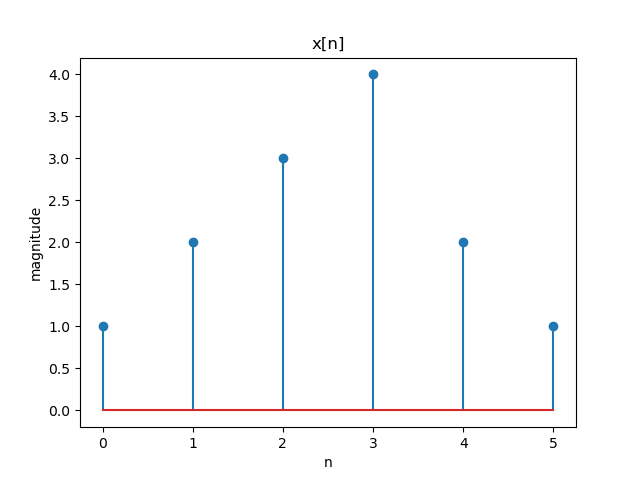
\includegraphics[height=6.8cm,width=9cm]{xn.png}
    \label{figs}
\end{figure}

\begin{figure}[h!]
    \centering
    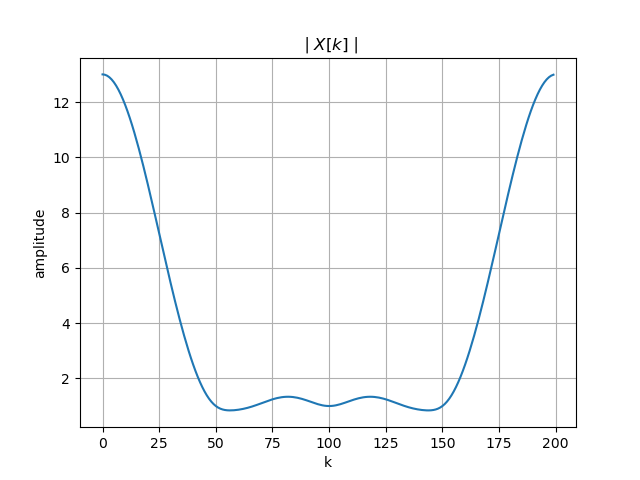
\includegraphics[height=6.8cm,width=9cm]{Xamp.png}
    \label{figs}
\end{figure}

\begin{figure}[h!]
    \centering
    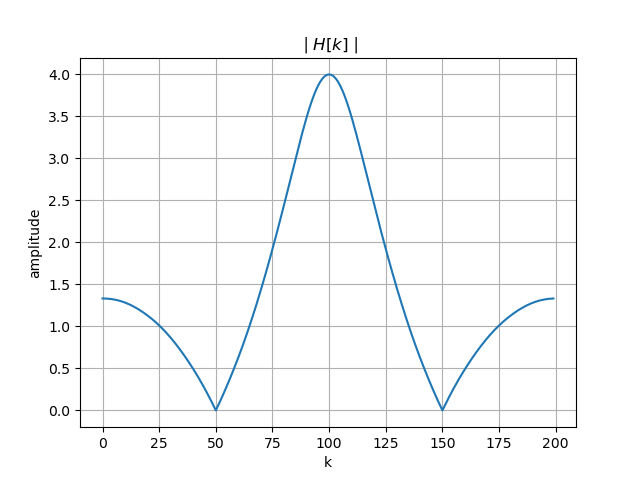
\includegraphics[height=6.8cm,width=9.25cm]{Hamp.png}
    \label{figs}
\end{figure}

\begin{figure}[h!]
    \centering
    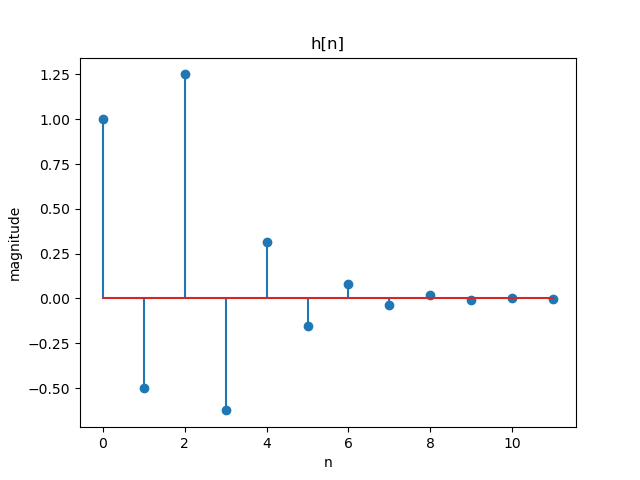
\includegraphics[height=6.8cm,width=9cm]{hn.png}
    \label{figs}
\end{figure}
\vspace{1cm}
\begin{figure}[h!]
    \centering
    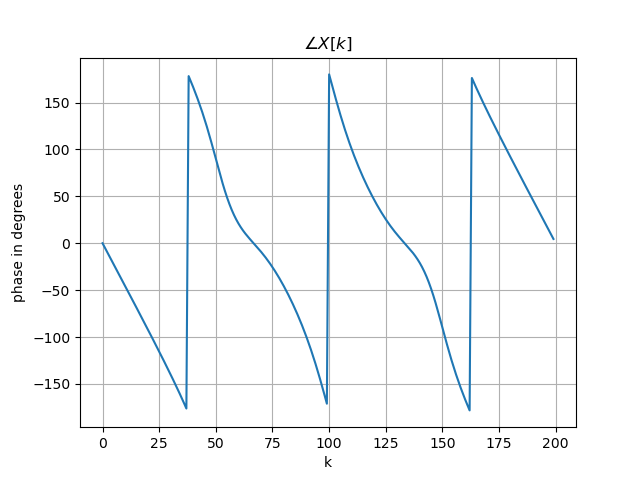
\includegraphics[height=6.8cm,width=9.5cm]{Xpha.png}
    \label{figs}
\end{figure}

\begin{figure}[h!]
    \centering
    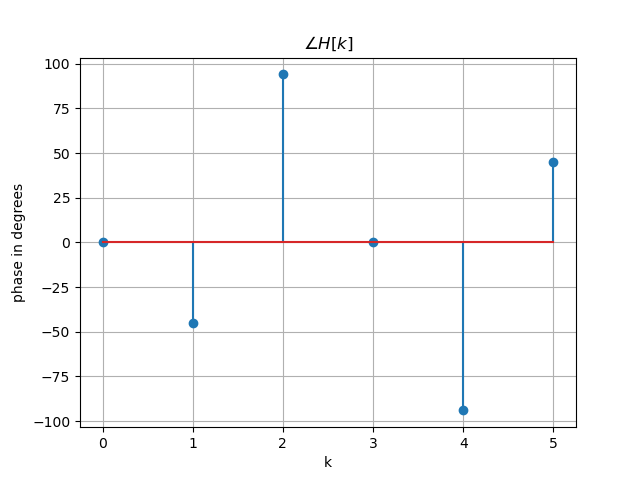
\includegraphics[height=6.8cm,width=9.5cm]{Hpha.png}
    \label{figs}
\end{figure}
\end{document}